\documentclass[11pt]{article}
\usepackage[margin=1in]{geometry}
\usepackage{amsmath,amssymb}
\usepackage{graphicx}
\usepackage{booktabs}
\usepackage[colorlinks=true,linkcolor=blue,citecolor=blue,urlcolor=blue]{hyperref}

% --- the only two lines to edit before submission ---
\newcommand{\authorname}{Singularity}
\newcommand{\affiliation}{}

\title{Wasserstein distances for wind-turbine power-curve monitoring:\\ a pre-specified simulation comparison}
\author{\authorname\\ \small \affiliation}
\date{\today}

\begin{document}
\maketitle

\begin{abstract}
Wind-turbine performance monitoring compares recent SCADA records with a healthy reference, usually through a binned
power curve or a residual statistic. These tools compare means; many faults instead change the \emph{shape} of the
distribution of power at a given wind speed. We compare five detectors on simulated 10-minute SCADA data with a fixed
false-alarm rate of 1\% per one-week window: the mean residual, a binned power-curve chi-square statistic, the
Kolmogorov--Smirnov statistic on residuals, the 1-Wasserstein distance between residual distributions, and a
1-Wasserstein distance conditional on wind speed. Four fault families at four severities were specified before the
single run: uniform derating, a shift of the power curve, a power cap and intermittent half-power operation.
Averaged over the twelve non-trivial scenarios, detection rates were 73\% (conditional Wasserstein), 71\% (residual
Wasserstein), 67\% (binned chi-square), 54\% (mean residual) and 28\% (Kolmogorov--Smirnov). The Wasserstein detectors
were best for derating and intermittent faults --- for example 81--83\% against 46\% at a 2\% intermittent share ---
while the binned chi-square was clearly best for a power cap (94\% against 62\% at a 5\% cap). No detector dominates;
the conditional Wasserstein distance is the best single choice in this benchmark and costs no more than a binned
power curve. Code and results are released.
\end{abstract}

\section{Introduction}
Supervisory control and data acquisition (SCADA) systems record wind speed and active power every ten minutes. The
standard way to see underperformance is to compare a recent power curve with a reference, either by bins of wind speed
as in IEC~61400-12-1 or through the residuals of a fitted curve. Distance-based variants compare a recent window with
a healthy model, for example with a Mahalanobis distance~\cite{Guo2022}, or track power-curve profiles over
time~\cite{Ding}. These statistics are built on means or on second moments. Faults such as intermittent curtailment,
controller limits or sporadic sensor errors change the \emph{distribution} of power at a given wind speed while
moving its mean only a little.

The Wasserstein distance~\cite{Villani} compares whole distributions and is sensitive to where probability mass moves
and how far. It is widely used in statistics and machine learning but, to our knowledge, it has not been evaluated as
a power-curve monitoring statistic. This study was prompted by an automated forecast that the method would enter
energy engineering; we test whether the transfer is useful, on a benchmark fixed in advance.

\section{Methods}
\paragraph{Simulated turbine.} Rated power $P_r=2$~MW; logistic power curve $P(v)=P_r/(1+e^{-0.9(v-9.5)})$ between
cut-in 3~m/s and cut-out 25~m/s; Weibull wind speeds (shape 2, scale 8~m/s); multiplicative noise with standard
deviation 4\% and additive noise of 1\% of $P_r$; power clipped to $[0,P_r]$.
\paragraph{Windows.} A healthy reference of four weeks (4032 records) and test windows of one week (1008 records).
\paragraph{Faults.} Derating $P\to(1-s)P$ with $s\in\{1,2,3,5\}\%$; curve shift $v_{50}\to v_{50}+s$ with
$s\in\{0.1,0.2,0.3,0.5\}$~m/s; power cap $P\to\min(P,(1-s)P_r)$ with $s\in\{2,5,8,12\}\%$; intermittent half power
for a share $s\in\{1,2,4,8\}\%$ of records.
\paragraph{Detectors.} Residuals are taken against the reference median power in 0.5~m/s bins.
(i) $|\bar r|$ over its standard error; (ii) $\sum_b n_b \bar r_b^2/\sigma_b^2$ over bins; (iii) the two-sample
Kolmogorov--Smirnov statistic between test and reference residuals; (iv) the 1-Wasserstein distance between the same
two residual samples; (v) the conditional distance $\sum_b n_b W_1(P_b^{\text{test}},P_b^{\text{ref}})/\sum_b n_b$,
where $P_b$ are the powers recorded in bin $b$.
\paragraph{Protocol.} Thresholds are the 99th percentile of each statistic over 1000 healthy test windows. Detection
rates are estimated on 300 faulty windows per scenario. All settings, including the random seed, were fixed before
the run, which was executed once.

\section{Results}
\begin{figure}[t]
\centering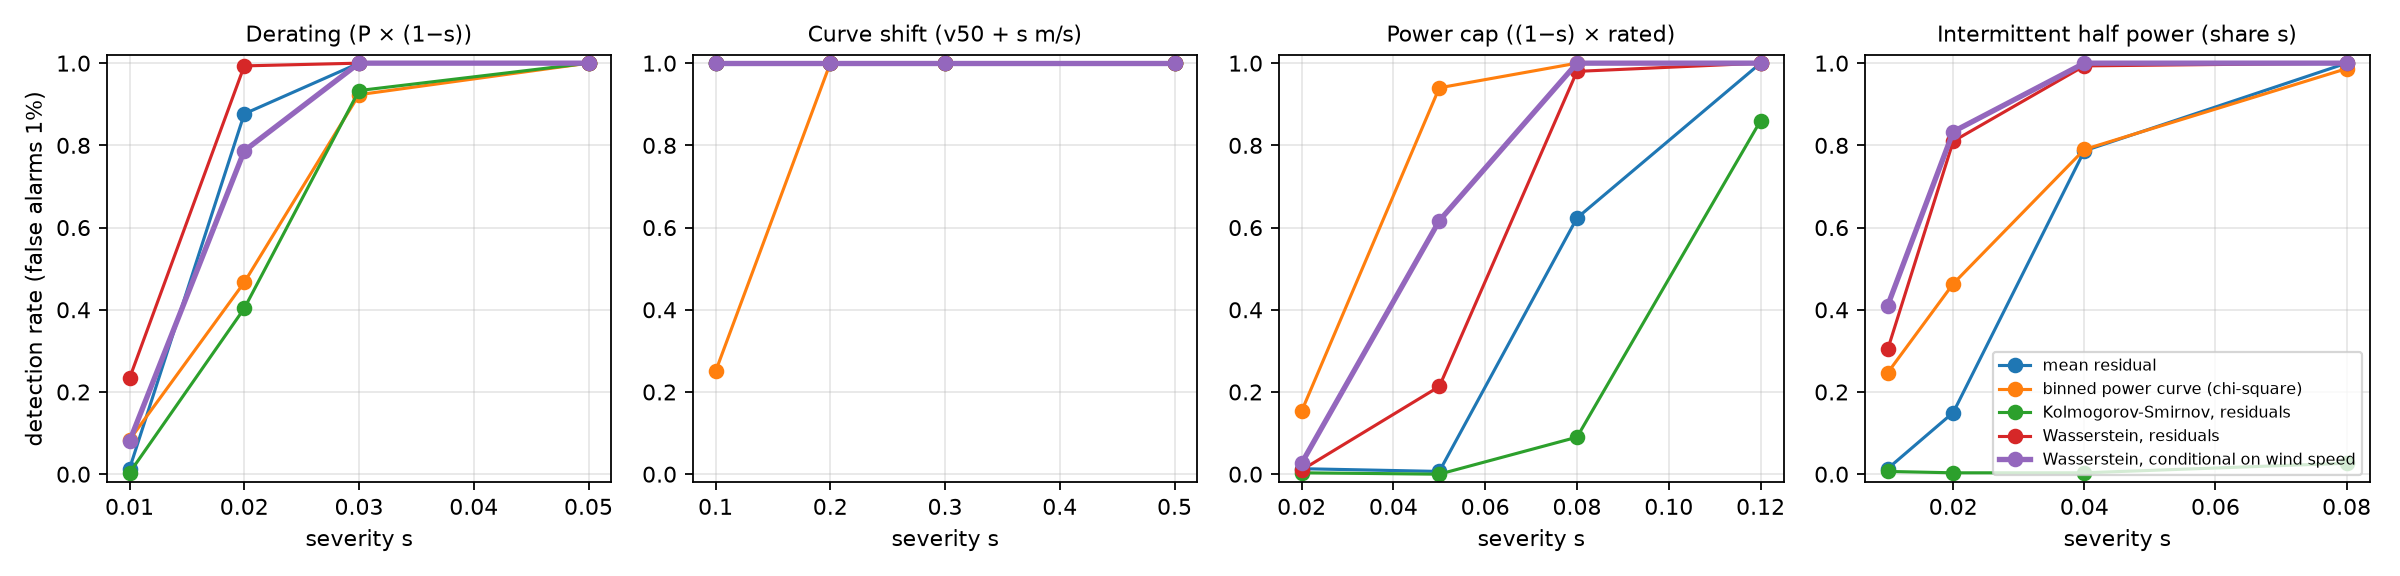
\includegraphics[width=\linewidth]{fig_power.png}
\caption{Detection rate at a 1\% false-alarm rate, by fault family and severity.}
\label{fig:power}
\end{figure}

\begin{table}[h]
\centering
\begin{tabular}{lcccc}
\toprule
detector & derating & power cap & intermittent & mean of 12 \\
\midrule
mean residual & 0.72 & 0.41 & 0.49 & 0.54 \\
binned chi-square & 0.62 & \textbf{0.77} & 0.62 & 0.67 \\
Kolmogorov--Smirnov & 0.58 & 0.24 & 0.01 & 0.28 \\
Wasserstein, residuals & \textbf{0.81} & 0.55 & 0.78 & 0.71 \\
Wasserstein, conditional & 0.72 & 0.66 & \textbf{0.81} & \textbf{0.73} \\
\bottomrule
\end{tabular}
\caption{Mean detection rate over the four severities of each family. The curve-shift family is detected by every
statistic from the smallest severity, except the binned chi-square at 0.1~m/s (25\%), and is omitted from the mean.}
\label{tab}
\end{table}

Figure~\ref{fig:power} and Table~\ref{tab} summarise the run. Three points stand out.
\begin{itemize}
\item \textbf{Shape-changing faults.} For intermittent half-power operation the Wasserstein detectors find a 2\% share
of affected records in 81--83\% of windows, against 46\% for the binned chi-square, 15\% for the mean residual and
0\% for Kolmogorov--Smirnov.
\item \textbf{Small derating.} At 2\% derating the residual Wasserstein distance detects 99\% of windows, against
88\% for the mean residual and 47\% for the binned chi-square.
\item \textbf{Where it loses.} A power cap acts only above rated wind speed, in few bins; the binned chi-square, which
weights each bin by its own variance, is clearly better there (94\% against 62\% at a 5\% cap).
\end{itemize}
The Kolmogorov--Smirnov statistic, which also compares distributions, performs poorly: it is driven by the largest
gap between cumulative distributions and ignores how far mass moves, which is exactly what the Wasserstein distance
measures.

\section{Discussion}
The conditional Wasserstein distance is a natural drop-in for a binned power curve: it uses the same bins and the same
reference, and replaces a comparison of bin means with a comparison of bin distributions. In this benchmark it is the
best single detector on average, and the residual version is the most sensitive to small uniform losses. A practical
monitor can combine it with the binned chi-square, which remains best for faults confined to a few bins.

\paragraph{Limitations.} The data are simulated, with independent records and a stationary wind climate; real SCADA
data have autocorrelation, seasonal air density, wake effects and data gaps, which change the null distribution and
call for block-bootstrap thresholds. The fault list is short and the severities were chosen by us. The next step is a
test on public SCADA data with logged faults.

\paragraph{Reproducibility.} \texttt{experiment.py} regenerates every number and figure; \texttt{results.json}
contains the output of the single run reported here.

\paragraph{Origin of the question.} The question came from an automated forecast (Singularity v3, registered on 5
November 2026 with a SHA-256 fingerprint) that the Wasserstein distance would enter the subfield \emph{Energy
Engineering and Power Technology}. The forecast concerned the arrival of the method, not the result of this study.

\begin{thebibliography}{9}
\bibitem{Guo2022} P.~Guo et al., Wind turbine performance degradation monitoring using DPGMM and Mahalanobis distance,
\emph{Renewable Energy} (2022).
\bibitem{Ding} Y.~Ding, \emph{Data Science for Wind Energy}, CRC Press (2019).
\bibitem{Villani} C.~Villani, \emph{Optimal Transport: Old and New}, Springer (2009).
\bibitem{IEC} IEC 61400-12-1, \emph{Power performance measurements of electricity producing wind turbines} (2017).
\end{thebibliography}
\end{document}
